% SPDX-FileCopyrightText: 2023 Iegor Riepin, Tom Brown
%
% SPDX-License-Identifier: CC-BY-4.0

\subsection{Methods and tools}

The simulations were carried out with the open-source software PyPSA for energy system modelling \cite{horschPyPSAEurOpenOptimisation2018} and Linopy for optimization \cite{LinopyLinearOptimization2024}.
The mathematical model is a system-wide cost-minimisation problem.
The objective of the model is to co-optimise (i) investment and dispatch decisions of generation and storage assets done by datacenters to meet their electricity demand in line with 24/7 CFE objectives, (ii) space-time load-shifting decisions subject to datacenter flexibility constraints, as well as (iii) investment and dispatch decisions of assets in the rest of the European electricity system to meet the demand of other consumers.
The model formulation includes the linear optimal power flow approximation for the transmission network based on the cycle-based formulation of Kirchhoff's Voltage Law \cite{horschLinearOptimalPower2018}. This work uses a brownfield investment approach, which means that the model includes information about the existing assets of the European electricity system.

The electricity system dispatch and investment problem of this type is a standard in the energy modelling literature \cite{OpenModelsWikib}. The clean computing model is based on the framework of 24/7 CFE accounting suggested by Google \cite{google-methodologies} that was implemented in realms of energy system models by Xu et al. \cite{xu-247CFE-report} and Riepin \& Brown \cite{riepinMeansCostsSystemlevel2023}. The space-time load flexibility model is inspired by the work of Zhang et al. \cite{zhangRemuneratingSpaceTime2022}. Finally, the space-time load flexibility as a degree of freedom within the 24/7 CFE matching problem is a novel contribution of this work.


\subsection{Datacenter model}

Datacenters are represented as a subset of demand nodes for electricity with a fixed demand profile, controlled degree of flexibility, and a set of specific constraints ensuring the carbon-free energy matching and utilisation of flexibility in a feasible domain.

% 24/7 CFE

The 24/7 CFE matching problem introduces a set of new model components (parameters, variables, constraints) into the power system optimisation problem to represent voluntary yet binding carbon-free energy matching commitments. Here, we model a situation where one company operates a network of datacenters that are geographically distributed but managed collectively. The company is committed \textit{to match every kilowatt-hour of electricity consumption by carbon-free sources in all datacenter locations}. To achieve the target, the company optimises its procurement of carbon-free generation and storage resources, dispatch of procured assets, imports of electricity from the regional grid, spatio-temporal load-shifting flexibility use (schematically illustrated in Figure \ref{fig:space-time-optimisation}), and when necessary, curtailment of excess generation.

\begin{figure}[b]
    \centering
    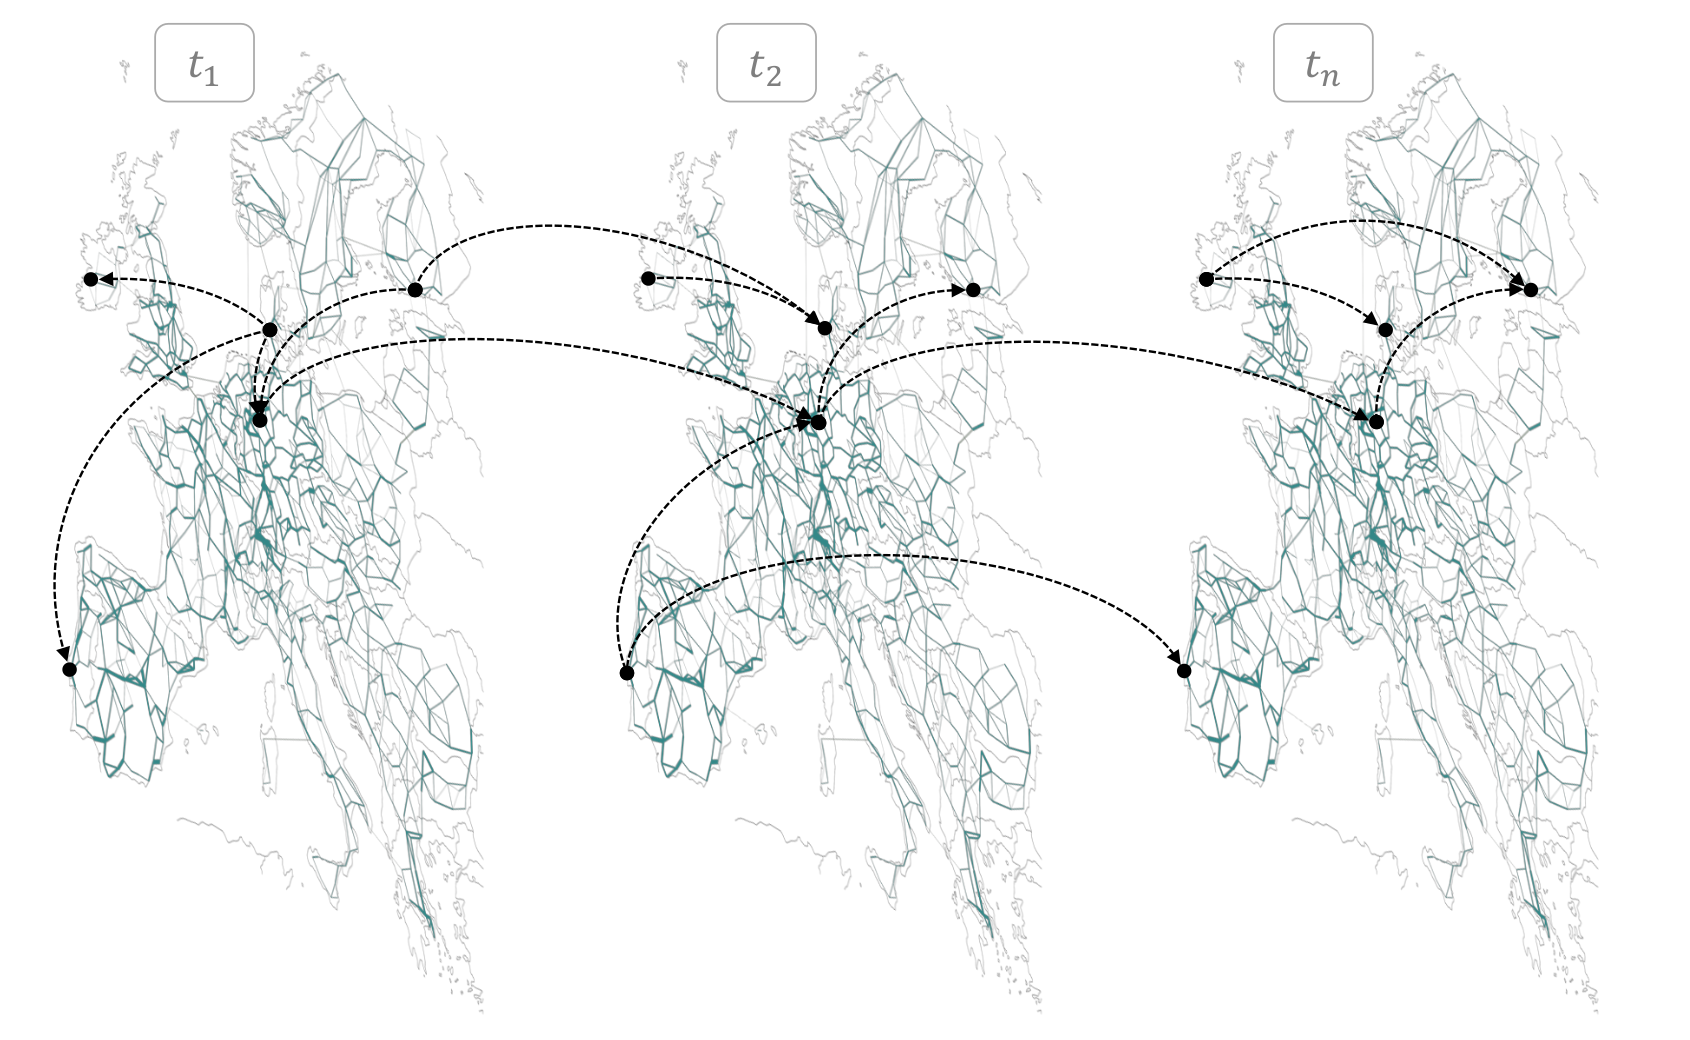
\includegraphics[width=1\columnwidth]{img/datacenter-problem.png}
    \caption{Illustration of spatio-temporal load-shifting optimisation problem faced by a datacenter operator.}
    \label{fig:space-time-optimisation}
\end{figure}

\textbf{A single datacenter with an inflexible load --} First, consider a case of a single datacenter with demand profile $d_{t}$ for each hour $t$ of the year. The demand profile is assumed to be known in advance and is not flexible. In such case, energy balance constraint requires that hourly demand is met by a combination of the following: (i) dispatch $g_{r,t}$ of procured carbon-free generators $r\in CFE$, (ii) discharge $\bar{g}_{s,t}$ and charge $\underline{g}_{s,t}$ of procured storage technologies $s\in STO$, and (iii) imports of electricity from the regional grid $im_{t}$:
\begin{equation}
    \begin{split}
        \sum_{r\in CFE} g_{r,t} &+ \sum_{s\in STO} \left(\bar{g}_{s,t} - \underline{g}_{s,t}\right) - ex_t + im_t = d_t \quad \forall t \in T
    \end{split}
\label{eqn:inflexnb}
\end{equation}
Note that if total electricity yield of renewable generators procured by the datacenter operator exceeds demand in a given hour, the excess electricity $ex_t$ has to be either stored or curtailed.\footnote{In practice, excess electricity can also be sold to the regional electricity market at wholesale market prices. This option is deliberately avoided in this work. When included, optimal usage of flexibility factors in potential revenues from selling excess electricity to the grid.}

The 24/7 CFE matching constraint requires that sum over hourly generation from the contracted generators, plus net dispatch of the storage technologies, plus imports of electricity from the regional grid multiplied by the grid's hourly CFE factor $CFE_t$ minus the excess electricity must be higher or equal than a certain CFE score $x$ multiplied by the total load of a datacenter:
\begin{equation}
    \begin{split}
        \sum_{r\in CFE, t\in T} g_{r,t} &+ \sum_{s\in STO, t\in T} \left(\bar{g}_{s,t} - \underline{g}_{s,t}\right) \\
        &- \sum_{t\in T} ex_t + \sum_{t\in T} CFE_t \cdot im_t \geq x \cdot \sum_{t\in T} d_t
    \end{split}
\label{eqn:CFE}
\end{equation}
% On CFE target
\noindent where \textit{CFE score} $x$[\%] measures the degree to which hourly electricity consumption is matched with carbon-free electricity generation \cite{google-methodologies}. Thus, equation (\ref{eqn:CFE}) allows for controlling \textit{the quality score} of the 24/7~CFE procurement by adjusting the parameter $x$, which was the subject of research in recent literature \cite{riepinMeansCostsSystemlevel2023,xu-247CFE-report}. Here, we focus on the best quality score ($x=1$) ensuring that every kilowatt-hour of electricity consumption is met by carbon-free sources at all times.

Note the following properties of the 24/7 CFE matching problem:

\begin{enumerate}
    \item The contracted generators $r\in CFE$ must be additional to the system and can be sited only in the local bidding zone, known as the requirements for \textit{additionality} and \textit{locational matching}.
    \item Excess electricity is not counted toward the CFE score and thus subtracted from the left-hand side of eq. (\ref{eqn:CFE}).
    \item The CFE factor of the regional grid ($CFE_t$) can be seen as the percentage of clean electricity in each MWh of imported electricity to supply demand of participating consumers in a given hour.
    To compute $CFE_t$, we consider both the hourly electricity mix in the local bidding zone and emission intensity of imported electricity from the neighbouring zones.
    The numerical simulations show that for the perfect 24/7 CFE matching ($x=1$), the datacenter operator does not rely on electricity imports from the regional grid because local electricity mix must have a strictly zero carbon content for imported electricity to be counted as \enquote{carbon-free}.
    Thus, the datacenter operator has one less degree of freedom to meet the 24/7 CFE matching target.
    The methodology to calculate the grid CFE factor and linearise resulting nonconvexity is described in detail in the prior work of the authors \cite{riepin-zenodo-systemlevel247}.
\end{enumerate}

\textbf{Multiple datacenters with flexible load --} Here we expand the 24/7 CFE matching problem to a case of multiple datacenters with flexible loads.

Let us assume that a known number of computing jobs with their associated power demand are \enquote{flexible}, i.e., power demand can potentially be shifted geographically across datacenter locations, or delayed to other times.\footnote{The amount of CPU usage on a cluster can be mapped accurately to electricity demand \cite{radovanovicIEEE2023}.} Thus, the \textit{dispatched load} $\widetilde{d}_t$ of a datacenter can deviate from the requested load $d_t$. The dispatched load $\widetilde{d}_t$ can take a value in a feasible domain that is constrained by a datacenter capacity (an upper limit) and the inflexible workloads volume (a lower limit), as illustrated in Figure \ref{fig:workloads}. The range of possible deviations between the dispatched and the requested loads is assumed to lie within a certain \textit{flexibility range} $f$~[\%], such as:
\begin{subequations}
  \begin{align}
    [1-f] \cdot d_t \le  \widetilde{d}_t  \le [1+f] \cdot d_t \quad \forall t \in T
    \label{eqn:dcaps} \\
    \widetilde{d}_t = d_t + (\overline{\Delta}_t - \underline{\Delta}_t) \quad \forall t \in T
    \label{eqn:dtilde}
  \end{align}
  \label{eqn:range}
\end{subequations}
\noindent where $\overline{\Delta}_t, \underline{\Delta}_t \in \mathbb{R}_{+}$ stand for positive/negative deviation of $\widetilde{d}_t$ and $d_t$ in hour $t$.

\begin{figure}
    \centering
    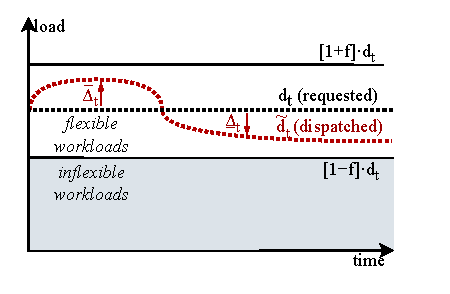
\includegraphics[width=1\columnwidth]{img/flexibility.pdf}
    \caption{Illustration of load flexibility concept: the absolute value of deviations between dispatched $\widetilde{d}_t$~[MW] and requested $d_t$~[MW] loads must fall within a certain flexibility range $f$~[\%] for each hour $t$.}
    \label{fig:workloads}
\end{figure}

% spatial shifting

To incorporate spatial flexibility, we use a concept of \textit{virtual links} representing non-physical pathways for shifting power loads across datacenter locations. Assume we have a set of datacenters $N$ located in various locations of an electricity network. Let $\Theta$ be the set of all virtual links and let $\delta_\vartheta \in \mathbb{R}_{+}$ be the spatial load shifts (flows via virtual pathways). We can thus define $\Theta_n^{snd} := \{\vartheta \in \Theta | snd(\vartheta) = n\} \subseteq \Theta$ and $\Theta_n^{rec} := \{\vartheta \in \Theta | rec(\vartheta) = n\} \subseteq \Theta$ to be the set of sending and receiving virtual links for each datacenter $n \in N$.

% temporal shifting

To incorporate temporal flexibility, we use a concept of \textit{temporal load management} that allows for shifting load from one time point to another in the future.\footnote{Zhang et al. \cite{zhangRemuneratingSpaceTime2022} show that the temporal load shifting problem can also be formulated via the concept of \textit{virtual links}. This yields the same mathematical problem.} Let each datacenter have a temporal load management mechanism $S_n^{dsm} := \{s' \in S | dsm(s') = n\}$. If $T = \{t_1 , t_2 , ..., t_T\}$ is a time horizon of our optimization problem, we can define $\bar{g}_{s',n,t}, \ubar{g}_{s',n,t} \in \mathbb{R}_{+}$ to be the amount of load shifted from time $t$ to another time point $t'$ for each datacenter $n \in N$ and $t, t' \in T$.

% new nodal balance

The nodal energy balance for inflexible consumers (eq.~\ref{eqn:inflexnb}) can now be extended by variables representing shifts of load \textit{in space} and \textit{in time}. Thus, the dispatched load  $\widetilde{d_{t}}$ of flexible consumer can deviate from the $d_{n,t}$ value due to space-time load shifting.
\begin{equation}
    \begin{split}
    &\sum_{r\in CFE} g_{r,n,t} + \sum_{s\in STO} \left(\bar{g}_{s,n,t} - \ubar{g}_{s,n,t}\right) - ex_{n,t} + im_{n,t}  = \\
    & d_{n,t} + \textcolor{darkred}{\sum_{\vartheta \in \Theta_n^{rec}}\delta_{\vartheta, t} - \sum_{\vartheta \in \Theta_n^{snd}}\delta_{\vartheta, t} + \sum_{{s'} \in S_n^{dsm}} \left(\bar{g}_{s',n,t} - \ubar{g}_{s',n,t}\right)} \\
    & \hspace{.5cm} \forall n \in N, t \in T
    \label{eqn:bothnb}
    \end{split}
\end{equation}
% computing capacity constraints
Computing capacity constraints (eq.~\ref{eqn:bothflex}) ensure that the dispatched load at each datacenter  $\widetilde{d}_{n,t}$ falls within the feasible domain considering both spatial and temporal load shifting. Computing capacity limit sets an upper bound (eq. \ref{eqn:bothb}) and inflexible workloads share sets a lower bound (eq. \ref{eqn:bothc}).
\begin{subequations}
    \begin{align}
      \begin{split}
        &\widetilde{d}_{n,t} =  d_{n,t} + \sum_{\vartheta \in \Theta_n^{rec}}\delta_{\vartheta, t} - \sum_{\vartheta \in \Theta_n^{snd}}\delta_{\vartheta, t} \\
        &+ \sum_{{s'} \in S_n^{dsm}} \left(\bar{g}_{s',n,t} - \ubar{g}_{s',n,t}\right) \quad \forall n \in N, t \in T \\
      \end{split}
      \label{eqn:botha} \\
      &\widetilde{d}_{n,t} \le [1+f] \cdot d_{n,t}  \quad \forall n \in N, t \in T \label{eqn:bothb} \\
      &\widetilde{d}_{n,t} \ge [1-f] \cdot d_{n,t}  \quad \forall n \in N, t \in T \label{eqn:bothc}
    \end{align}
    \label{eqn:bothflex}
\end{subequations}
Note that spatial load shifts are not subject to any electricity network transmission constraints. As such, the only source of congestion for the virtual links is computing capacity constraints (i.e., availability of flexible workloads) as defined in eq. (\ref{eqn:bothflex}).

Temporal load shifts have an additional constraint ensuring that the cluster-level compute usage is preserved within a certain time interval. We follow the work of Radovanovic et al. \cite{radovanovicIEEE2023} and implement a \textit{daily} compute usage conservation rule:
\begin{equation}
    \sum_{t | t \in t(DAYS)} \left(\bar{g}_{s',t} - \ubar{g}_{s',t}\right) = 0 \quad \forall {s'} \in S_n^{dsm}
    \label{eqn:dailyconserv2}
\end{equation}
% 24/7 CFE matching with flexible load
Finally, the 24/7~CFE matching constraint defined in eq. \ref{eqn:CFE} can be defined over a set of datacenters nodes $N$ and extended on the right-hand side with variables representing spatial and temporal load shifts:
\begin{align}
    &\sum_{r\in CFE, t\in T} g_{r,n,t} + \sum_{s\in STO, t\in T} (\bar{g}_{s,n,t} - \ubar{g}_{s,n,t}) \nonumber \\
    &- \sum_{t\in T} ex_{n,t} + \sum_{t\in T} CFE_{n,t} \cdot im_{n,t} \geq \nonumber \\
    &x_n \cdot
        \Bigg( \sum_{t\in T} \Big( d_{n,t} + \textcolor{darkred}{\sum_{\vartheta \in \Theta_n^{rec}}\delta_{\vartheta, t} - \sum_{\vartheta \in \Theta_n^{snd}}\delta_{\vartheta, t}} \nonumber \\
        & \textcolor{darkred}{+ \sum_{{s'} \in S_n^{dsm}} (\bar{g}_{s',n,t} - \ubar{g}_{s',n,t})}\Big)\Bigg) \quad \forall n \in N\label{eqn:bothCFE}
\end{align}
Overall, the mathematical formulation of the 24/7 CFE matching problem extended with eqs. \ref{eqn:bothnb}-\ref{eqn:bothCFE} represents a situation where a company pursuing the 24/7 CFE matching target has two additional degrees of freedom---the ability to shift power loads in space and in time---as part of its decision-making process. Co-optimisation of space-time load-shifting flexibility with procurement and dispatch of carbon-free generators can lead to a more resource-efficient and cost-effective solution for carbon-free electricity matching.

\subsection{Model scope and parametrisation}

Geographical focus of the model covers the entire European electricity system clustered to 37 zones. Each zone represents an individual country. Some countries that straddle different synchronous areas are split to individual bidding zones, such as DK1 (West) and DK2 (East). A set of datacenters---electricity consumers committed to 24/7 CFE goals---are placed in several selected zones in each scenario. Each zone have unique weather patterns, renewable potentials, and background electricity mixes. The model's time horizon spans one year. All model runs are done with 1-hourly temporal resolution, i.e., 8760 time steps.

We assume all datacenters to have a load of 100~MW and a flat (baseload) consumption profile. Note that the shape of a consumption profile does not significantly impact the costs of the 24/7 CFE matching \cite{riepin-zenodo-systemlevel247}. We assume a \textit{complete graph} superstructure of virtual links. Specifically, for every pair of distinct datacenters \(n, m \in N\) where \(n \neq m\), there exists a bidirectional virtual link \(\vartheta_{nm} \in \Theta\) such that \(snd(\vartheta_{nm}) = n\) and \(rec(\vartheta_{nm}) = m\), and conversely, \(snd(\vartheta_{mn}) = m\) and \(rec(\vartheta_{mn}) = n\). This configuration ensures that each datacenter is capable of both sending and receiving spatial load shifts to and from every other datacenter in the network.

The model is parametrised for the exemplary year 2025. Input data such as technology cost assumptions, national renewable policies, decommissioning of legacy power plant fleet, and system-wide assumptions are parametrised accordingly. For the 24/7 CFE matching problem, we assume a set of energy technologies that \textit{are commercially available today}: onshore wind, utility scale solar photovoltaics (\gls{PV}), and battery storage. Cost and other assumptions for these technologies are collected from the Danish Energy Agency \cite{DEA-technologydata} and provided in \nameref{sec:si}.

Weather-dependent power potentials for renewable energy technologies, including those of solar PV and onshore wind generators available for the 24/7 CFE matching, are simulated with hourly temporal resolution using the ERA5 reanalysis dataset \cite{hersbachERA5GlobalReanalysis2020} using the open-source tool Atlite \cite{atlite-github}. We assume 2013 to be a representative climate year.

Other electricity system data is processed with an open-source model for the European energy system PyPSA-Eur \cite{PyPSAEur-docs}. All code and input data to reproduce the experiments are available at the GitHub repository under open licenses \cite{github-spacetime}.


